\subsection{Calibration of the cars}
When the server, vehicles and client were implemented, and the second vehicle built, we did some testing to figure out how the car’s behaved when given directions by the server. In this test the vehicles were given a specific velocity and driving distance by the server. When the vehicles arrived at their destination the server would tell them to stop. The car’s drove in a straight line.

The vehicles were able to send information, and respond correctly to the servers commands. We also observed that the vehicles drove a different length for each velocity given even though the length was the same. This is because the velocity given to the vehicles is the amount of power going into the car’s motors, not the actual velocity of the car’s. We wanted the demo to be accurate so our group did some further testing where we wrote down the results. 

\begin{table}
	\begin{center}
		\begin{tabular}{rrrr}
			\hline
			Power (?) & Length (cm) & Time (s) & Velocity (cm/s) \\
			\hline
			40 & 467 & 8.98 & 52.00 \\
			50 & 425 & 7.28 & 58.38 \\
			60 & 400 & 6.06 & 66.01 \\
			70 & 357 & 5.18 & 68.92 \\
			80 & 325 & 4.49 & 72.32 \\
			90 & 314 & 4.03 & 77.92 \\
			100 & 286 & 3.62 & 79.01 \\
			\hline
		\end{tabular}
		\caption{Test text}
	\end{center}
\end{table}

The data Power was the velocity given by the server. Velocity was the actual velocity in our testing, which is length divided by time. As you can see the velocity was not the same as the power. We then made a graph to visualize the two values. The $y$-axis was the velocity while the $x$-axis is the power.

\begin{figure}[h!]
		\centering
	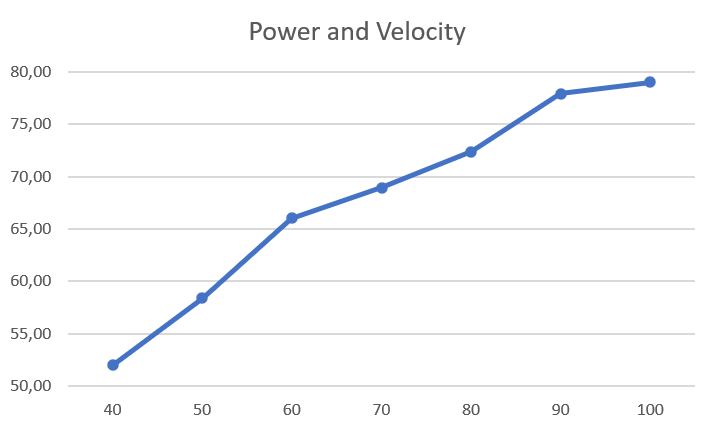
\includegraphics[width=1\linewidth]{figures/velocity_and_power}
	\caption[Graph of velocity as function of power]{Graph of velocity as a function of power}
	\label{fig:graphvelpow}
\end{figure}

We observed that the correlation between power and velocity seemed linear. This means we could make a specific formula that describes the correlation between the two values. We used linear regression to figure out this formula:

\begin{figure}[h!]
	\centering
	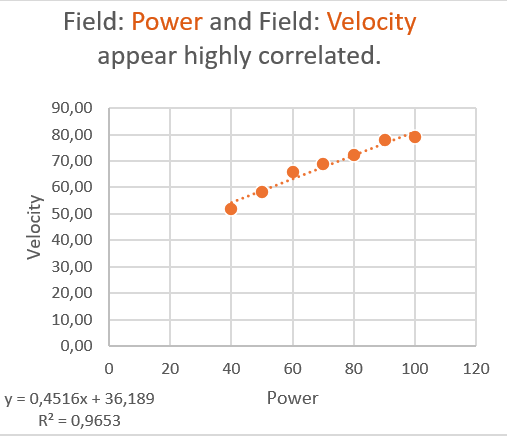
\includegraphics[width=1\linewidth]{figures/function_of_power}
	\caption{Graph of velocity as a function of power with linear regression}
	\label{fig:functionofpower}
\end{figure}


The formula we ended up with was as follows: $v(P) = 0.4516\cdot P + 36.189$, where $P$ is power and $v$ is velocity, with a mean square error of $R^2=0.9653$. When we coded the formula into the vehicles we did another set of testing. We observed that the vehicles drove more or less the same distance for each power given. If we wanted an even more accurate formula we could have tuned the formula with the test results from our new test. Although the results were not hundred percent accurate, we concluded it was accurate enough for our demonstration. 

To test the solution we have worked on, we made a physical demonstration with two cars that meet at an intersection, as part of the product documentation. We want to test that a combination of a centralized communication system and artificial intelligence can improve traffic flow. What we wanted to observe was if the velocity of the vehicles were not drasticly changed and therefore not distrupting the traffic flow.

